\documentclass{ctexart}

\usepackage[x11names]{xcolor}   % 颜色
\usepackage{amsmath, amssymb}   % 数学公式与符号
\usepackage{hyperref}           % 超链接
\usepackage{graphicx}           % 插图
\usepackage{lmodern, bm}        % 额外字体与粗体样式
\usepackage{calc}               % 支持不同单位的长度计算
\usepackage{array}
\usepackage{geometry}
\usepackage{amsthm}
\usepackage{graphicx}
\hypersetup{colorlinks = true}

\setlength{\lineskiplimit}{2.5pt}
\setlength{\lineskip}{4pt}

\newcommand{\Romannumeral}[1]{\MakeUppercase{\romannumeral #1}}
\newcommand{\Pblock}[1]{\fbox{\parbox{\textwidth-28pt}{#1}}}
\makeatletter
\newcommand{\defeq}{\mathrel{\rlap{%
                     \raisebox{0.3ex}{$\m@th\cdot$}}%
                     \raisebox{-0.3ex}{$\m@th\cdot$}}%
                     =}
\makeatother

\newcommand{\dif}{\mathop{}\!\mathrm{d}}

% 定义两个计数器:“定义” 和 “定理”
\newcounter{definition}[subsection]
\newcounter{subdefinition}[definition]
\newcounter{theorem}[subsection]
\newcounter{subtheorem}[theorem]

\NewDocumentEnvironment{definition}{o}{\IfNoValueTF{#1}{\stepcounter{definition}\textbf{定义\,\thedefinition.}}{\stepcounter{definition}\textbf{定义\,\thedefinition\,(#1).}}}{}
\NewDocumentEnvironment{subdefinition}{o}{\IfNoValueTF{#1}{\stepcounter{subdefinition}\textbf{定义\,\thedefinition.\thesubdefinition.}}{\stepcounter{subdefinition}\textbf{定义\,\thedefinition.\thesubdefinition\,(#1).}}}{}

\NewDocumentEnvironment{theorem}{o}{\IfNoValueTF{#1}{\stepcounter{theorem}\textbf{定理\,\thetheorem.}}{\stepcounter{theorem}\textbf{定理\,\thetheorem\,(#1).}}}{}
\NewDocumentEnvironment{subtheorem}{o}{\IfNoValueTF{#1}{\stepcounter{subtheorem}\textbf{定理\,\thetheorem.\thesubtheorem.}}{\stepcounter{subtheorem}\textbf{定理\,\thetheorem.\thesubtheorem\,(#1).}}}{}

\title{吉米多维奇习题集部分解答}
\author{陈程}
\date{\today}

\begin{document}
\maketitle

\tableofcontents

\section{分析引论}
\subsection{实数}
\textbf{6.} 证明伯努利不等式:
\[\prod_{i=1}^{n} (1 + x_i) \geqslant 1 + \sum_{i=1}^{n} x_i \tag{6.1}\]
式中 $x_1, x_2, \cdots, x_n$ 是符号相同且大于 $-1$ 的数.
\begin{proof}
    运用数学归纳法,当 $n$ 等于 1 的时候不等式显然成立.

    假设 $n = k$ 时不等式 $(6.1)$ 成立,即
    \[\prod_{i=1}^{k} (1+x_i) \geqslant 1 + \sum_{i=1}^{k} x_i \tag{6.2}\]

    则
    \[\prod_{i=1}^{k+1} (1+x_i) \geqslant 1 + \sum_{i=1}^{k+1} x_i \tag{6.3}\]
    \[\Leftrightarrow (1 + x_{k+1}) \cdot \prod_{i=1}^{k}(1+x_i) \geqslant 1 + \sum_{i=1}^{k}x_i + x_{k+1}\]
    \[\Leftarrow (1 + x_{k+1}) \cdot \left(1 + \sum_{i=1}^{k}x_i\right) \geqslant 1 + \sum_{i=1}^{k}x_i + x_{k+1}\]
    \[\Leftrightarrow x_{k+1} \cdot \left(1 + \sum_{i=1}^{k}x_i\right) \geqslant x_{k+1}\]
    \[\Leftrightarrow x_{k+1}\sum_{i=1}^{k}x_i \geqslant 0 \tag{6.4}\]
    即当 $n = k+1$ 时不等式 $(6.1)$ 成立.
\end{proof}\vspace{9pt}

\textbf{8.} 证明不等式:
\[n! < \left(\frac{n+1}{2}\right)^n \quad (n > 1) \tag{8.1}\]
\begin{proof}
    令
    \[A_n = n! \quad B_n = \left(\frac{n+1}{2}\right)^n\]
    则原不等式 $(8.1)$ 等价于
    \[A_n < B_n \quad (n>1) \tag{8.2}\]

    又因为 $A_n, B_n$ 恒为正数,$A_2 = 2 < 9/4 = B_2$,因此式 $(8.2)$
    \[\Leftarrow \frac{A_{n+1}}{A_n} < \frac{B_{n+1}}{B_n} \quad (n>1) \tag{8.3}\]
    \[\Leftrightarrow n+1 < \frac{n+2}{2} \cdot \left(\frac{n+2}{n+1}\right)^n \quad (n>1)\]
    \[\Leftrightarrow 2 < \left(\frac{n+2}{n+1}\right)^{n+1} \quad (n>1)\]
    \[\Leftrightarrow 2 < \left(1 + \frac{1}{n+1}\right)^{n+1} \quad (n>1) \tag{8.4}\]
\end{proof}\vspace{9pt}

\textbf{9.} 证明不等式:
\[\prod_{i=1}^{n}(2i)! > [(n+1)!]^n \quad (n>1) \tag{9.1}\]
\begin{proof}
    不等式 $(9.1)$
    \[\Leftarrow (2n+2)! > \frac{[(n+2)!]^{n+1}}{[(n+1)!]^n} \quad (n>1) \tag{9.2}\]
    \[\Leftrightarrow (2n+2)! > (n+2)!(n+2)^n \quad (n>1)\]
    \[\Leftarrow (2n+3)(2n+4) > (n+3) \cdot \frac{(n+3)^{n+1}}{(n+2)^n} \quad (n>1) \tag{9.3}\]
    \[\Leftrightarrow 2 \cdot \frac{2n+3}{n+2} > \left(\frac{n+3}{n+2}\right)^{n+2} \quad (n>1)\]
    \[\Leftrightarrow 2 \cdot \left(2 - \frac{1}{n+2}\right) > \left(1 + \frac{1}{n+2}\right)^{n+2} \quad (n>1)\]
    \[\Leftarrow 2 \cdot \left(2 - \frac{1}{n+2}\right) > 3 > \left(1 + \frac{1}{n+2}\right)^{n+2} \quad (n>1) \tag{9.4}\]
\end{proof}\vspace{9pt}

\textbf{10.} 证明不等式:
\[\left\vert \sin \left(\sum_{k=1}^{n}x_k\right)\right\vert \leqslant \sum_{k=1}^{n} \sin x_k \quad (0 \leqslant x_k \leqslant \pi, k = 1,2,\cdots,n) \tag{10.1}\]
\begin{proof}
    运用数学归纳法,当 $n=1$ 时不等式 $(10.1)$ 显然成立.

    假设当 $n = p$ 时不等式 $(10.1)$ 成立,即
    \[\left\vert \sin \left(\sum_{k=1}^{p}x_k\right)\right\vert \leqslant \sum_{k=1}^{p} \sin x_k \tag{10.2}\]
    则
    \begin{align*}
        \left\vert \sin \left(\sum_{k=1}^{p+1}x_k\right)\right\vert &= \left\vert \sin\left(x_{p+1} + \sum_{k=1}^{p}x_k\right)\right\vert\\
        &=\left\vert \sin (x_{p+1}) \cos \left(\sum_{k=1}^{p}x_k\right) + \sin \left(\sum_{k=1}^{p}x_k\right) \cos (x_{p+1})\right\vert\\
        &\leqslant \left\vert\sin (x_{p+1}) \cos \left(\sum_{k=1}^{p}x_k\right)\right\vert + \left\vert\sin \left(\sum_{k=1}^{p}x_k\right) \cos (x_{p+1})\right\vert\\
        &\leqslant \sin x_{p+1} + \left\vert \sin \left(\sum_{k=1}^{p}x_k\right)\right\vert\\
        &\leqslant \sin x_{p+1} + \sum_{k=1}^{p} \sin x_k\\
        &= \sum_{k=1}^{p+1} \sin x_k\\
    \end{align*}
\end{proof}
\vspace{9pt}

\textbf{11.} 设 $c$ 为正整数,而不为整数的平方,且 $A/B$ 为确定实数 $\sqrt{c}$ 的分割,其中 $B$ 类包含所有满足 $b^2 > c$ 的正有理数 $b$,而 $A$ 类包含所有其余的有理数. 求证:在 $A$ 类中无最大数,而在 $B$ 类中无最小数.
\begin{proof}
    引理:对于正整数 $c$,如果 $\sqrt{c}$ 不是整数,则不存在有理数 $x$ 使得 $x^2 = c$.

    所以 $\forall a \in A \cap \mathbb{Q}^+: a^2 < c$.

    如果 $A$ 类中有最大数 $a$,则可以验证
    \[\left(\frac{c-1}{\frac{c-1}{a+1}+2}+1\right)^2 < c\]
    所以 $\displaystyle \frac{c-1}{\frac{c-1}{a+1}+2}+1 \in A$.

    也可以验证
    \[\frac{c-1}{\frac{c-1}{a+1}+2}+1 > a\]
    这与 $a$ 是 $A$ 中最大数矛盾.

    同理,$B$ 中也没有最小数.
\end{proof}
附记:这里解释一下为什么会出现 $\displaystyle \frac{c-1}{\frac{c-1}{a+1}+2}+1$ 这个看起来很奇怪的表达式,这个表达式源于一种用有理数迭代估计无理数的方法.

这里以估计 $\sqrt{3}$ 为例.

$\sqrt{3}$ 是方程 $x^2 = 3$ 的一个(正)根,将方程变形成
\[(x-1)(x+1) = 2\]
\[x = \frac{2}{x+1}+1\]

我们构造一个数列 $\{x_n\}$,令 $x_1 = 1$,$\displaystyle x_{n+1} = \frac{2}{x_n+1}+1$. 这个数列的极限就是 $\sqrt{3}$(当然要先验证这个数列的极限存在). 这里给出该数列的前 $10$ 项:

\begin{center}
    \begin{tabular}{c|cccccccccc}
        \hline
        $n$ & $1$ & $2$ & $3$ & $4$ & $5$ & $6$ & $7$ & $8$ & $9$ & $10$\\
        $a_n$ & 2 & 1.6667 & 1.75 & 1.7273 & 1.7333 & 1.7317 & 1.7321 & 1.7320 & 1.7321 & 1.7321\\
        \hline
    \end{tabular}
\end{center}

可以看到,数列的项一半小于根号三,一半大于根号三,交错排布,$\lvert x_n - \sqrt{3}\rvert$ 单调递减(可以用代数严格证明),因此只要一次迭代两步,即 $\displaystyle x_{n+2} = \frac{2}{\frac{2}{x_n+1}+2}+1$ 就能满足第 $10$ 题的要求.

类似的,也可以通过方程
\[x^3 = 3\]
\[\rightarrow (x-1)(x^2+x+1) = 2\]
\[\rightarrow x = \frac{2}{x^2+x+1}+1\]
来构造数列满足 $\displaystyle x_{n+1} = \frac{2}{x_n^2+x_n+1}+1$ 来估计 $\sqrt[3]{3}$.

\subsection{数列理论}
\textbf{49.} 求极限
\[\lim_{n \rightarrow \infty} \frac{(-2)^n + 3^n}{(-2)^{n+1} + 3^{n+1}} \tag{49.1}\]
\begin{proof}
    令
    \[A_n = \frac{(-2)^n + 3^n}{(-2)^{n+1} + 3^{n+1}} \tag{49.2}\]
    易得对于任意的正整数 $n$,
    \[A_n > 0\]

    所以数列 $A_n$ 与数列 $\sqrt[n]{A_1A_2 \cdots A_n}$ 拥有相同的极限(两者的极限要么同时存在,要么都不存在),而
    \[\lim_{n \rightarrow \infty} \sqrt[n]{A_1 A_2 \cdots A_n} = \lim_{n \rightarrow \infty} \sqrt[n]{\frac{1}{(-2)^{n+1} + 3^{n+1}}} = \frac{1}{3} \cdot \left(\lim_{n \rightarrow \infty} \sqrt[n]{(-2/3)^{n+1} + 1}\right)^{-1} = \frac{1}{3} \tag{49.3}\]

    所以数列 $A_n$ 的极限存在而且极限为 $1/3$.
\end{proof}\vspace{9pt}

\textbf{55.} 求极限
\[\lim_{n \rightarrow \infty} \left(\frac{1}{2} + \frac{3}{2^2} + \frac{5}{2^3} \cdots + \frac{2n-1}{2^n}\right)\]
\begin{proof}
    对级数进行分组,
    \[\sum_{k=1}^{n} \frac{2k-1}{2^k} = \sum_{k=1}^{n} \frac{2k}{2^k} - \sum_{k=1}^{n} \frac{1}{2^k} = \sum_{k=1}^{n}\sum_{j=1}^{k}\frac{2}{2^k} - \sum_{k=1}^{n} \frac{1}{2^k} = \sum_{j=1}^{n} \sum_{k=j}^{n} \frac{2}{2^k} - \sum_{k=1}^{n}\frac{1}{2^k}\]

    易得
    \[\lim_{n \rightarrow \infty} \sum_{k=1}^{n} \frac{1}{2^k} = 1\]
    \[\lim_{n \rightarrow \infty} \sum_{j=1}^{n}\sum_{k=j}^{n} \frac{2}{2^k} = \lim_{n \rightarrow \infty} \sum_{j=1}^{n} \left(\lim_{n \rightarrow \infty} \sum_{k=j}^{n} \frac{2}{2^k}\right) = \lim_{n \rightarrow \infty} \sum_{j=1}^{n} \frac{4}{2^j} = 4\]

    所以
    \[\lim_{n \rightarrow \infty} \sum_{k=1}^{n} \frac{2k-1}{2^k} = 4 - 1 = 3\]
\end{proof}\vspace{9pt}

\newpage
\textbf{奇思妙想:}对于一个给定的二元函数\footnote{默认为实值函数,但是下面的论述也能推广到复数域上去} $A$,下面两个极限在什么情况下相等(在下列极限都存在的情况下考虑)?
\[\lim_{n \rightarrow \infty} \sum_{i=1}^{n}\sum_{j=i}^{n} A(i;j) = \sum_{i=1}^{\infty} \left(\sum_{j=i}^{\infty} A(i;j)\right)\]

\begin{proof}
    因为
    \begin{align*}
        \lim_{n \rightarrow \infty} \sum_{i=1}^{n}\sum_{j=i}^{n} A(i;j) &= \lim_{n \rightarrow \infty} \sum_{i=1}^{n} \left(\sum_{j=i}^{\infty} A(i;j) - \sum_{j=n+1}^{\infty} A(i;j)\right)\\
        &= \lim_{n \rightarrow \infty} \sum_{i=1}^{n} \left(\sum_{j=i}^{\infty} A(i;j)\right) - \lim_{n \rightarrow \infty} \sum_{i=1}^{n} \left(\sum_{j=n+1}^{\infty} A(i;j)\right)\\
        &= \sum_{i=1}^{\infty} \left(\sum_{j=i}^{\infty} A(i;j)\right) - \lim_{n \rightarrow \infty} \sum_{i=1}^{n} \left(\sum_{j=n+1}^{\infty} A(i;j)\right)
    \end{align*}
    
    所以两个极限相等只要
    \[\lim_{n \rightarrow \infty} \sum_{i=1}^{n} \left(\sum_{j=n+1}^{\infty} A(i;j)\right) = 0\]

    其中 $\displaystyle \sum_{j=n+1}^{\infty} A(i;j)$ 可以看作无穷级数 $\displaystyle \sum_{j=1}^{\infty} A(i;j)$ 的\emph{余项},用 $R(i;n)$ 来表示.
    
    所以把
    \[\sum_{i=1}^{n} R(i;n)\]
    看作是一个关于 $n$ 的数列,只要在 $n \rightarrow \infty$ 时它是 $o(1)$ 即可.
    
    然后定义
    \[B_n \defeq \sup\Bigl\{\bigl| R(i;n)\bigr| \Bigm| i \leqslant n\Bigr\}\]
    
    有
    \[\left|\sum_{i=1}^{n} R(i;n)\right| \leqslant n \cdot B_n\]
    
    只要 $B_n$ 在 $n \rightarrow \infty$ 时是 $\displaystyle o\biggl(\frac{1}{n}\biggr)$ 即可.

    现在我们考虑对于任意的 $i$,$R(i;n) = o(1/n)$ 这一特殊情况
    \[C(i;n) \defeq \sup\Bigl\{ \bigl| R(i;j) \bigr| \Bigm| j \geqslant n\Bigr\}\]

    我猜测在这种情况下原命题成立的一个充分条件为 $C(n;n) = o(1/n)$,现在尝试证明.

    因为当 $n \rightarrow \infty$ 时
    \[\forall i \in \mathbb{N}^*: R(i;n) = o(1/n)\]

    所以
    \[\forall i \in \mathbb{N}^*: C(i;n) = o(1/n)\]
    \[\forall k \in \mathbb{N}^*: \forall \varepsilon > 0: \exists N \in \mathbb{N}^*: \forall n > N: \forall i \leqslant k: C(i;n) < \frac{\varepsilon}{n} \tag{1}\]

    因为 $C(n;n) = o(1/n)$,所以
    \[\forall \varepsilon > 0: \exists k \in \mathbb{N}^*: \forall n > k: C(n;n) < \frac{\varepsilon}{n} \tag{2}\]

    再加上
    \[\forall n \in \mathbb{N}^*: \left|\sum_{i=1}^{n}R(i;n)\right| \leqslant \sum_{i=1}^{n} C(i;n) \leqslant \sum_{i=1}^{k} C(i;n) + \sum_{i=k+1}^{n} C(i;i) \tag{3}\]
    
    有
    \[\forall \varepsilon > 0: \exists k \in \mathbb{N}^*: \exists N \in \mathbb{N}^*: \forall n > \max\{k, N\}: \left|\sum_{i=1}^{n}R(i;n)\right| < k \cdot \frac{\varepsilon}{n} + (n-k) \cdot \frac{\varepsilon}{n} = \varepsilon\]

    所以
    \[\lim_{n \rightarrow \infty} \sum_{i=1}^{n} R(i;n) = 0\]

    得证.

    这里可以给几个具体例子来参考

    \[A(i;j) = (-1)^{j-i} \cdot 2^{-\lfloor{(j-i)/2}\rfloor}\]
    \[A(i;j) = 2^{-j}\]
    \[A(i;j) = \frac{1}{j} - \frac{1}{j+1}\]
\end{proof}\vspace{9pt}

\textbf{70.} 证明:
\[0 < \mathrm{e} - \left(1 + \frac{1}{n}\right)^n < \frac{3}{n} \quad (n = 1,2,\cdots) \tag{70.1}\]
\begin{proof}
    先证明引理:
    \[\left(1+\frac{1}{n}\right)^n < \mathrm{e} < \left(1+\frac{1}{n}\right)^{n+1} \quad (n = 1,2,\cdots) \tag{70.2}\]

    对于数列 $\displaystyle \left\{\left(1 + \frac{1}{n}\right)^n\right\}$,因为
    \begin{align*}
        \frac{[1+1/(n+1)]^{n+1}}{(1+1/n)^n} &= \left(\frac{n}{n+1}\right)^n \cdot \left(\frac{n+2}{n+1}\right)^{n+1}\\
        &= \left(1 - \frac{1}{(n+1)^2}\right)^{n+1} \cdot \left(\frac{n+1}{n}\right)\\
        &> \left(1 - \frac{1}{n+1}\right) \cdot \left(\frac{n+1}{n}\right)\\
        &= 1
    \end{align*}

    所以 $\displaystyle \left\{\left(1 + \frac{1}{n}\right)^n\right\}$ 是单调增数列,即
    \[\left(1+\frac{1}{n}\right)^n < \lim_{n \rightarrow \infty} \left(1+\frac{1}{n}\right)^n = \mathrm{e}\]

    不等式 $(70.2)$ 另一边的证明同理.

    所以
    \[0 < \mathrm{e} - \left(1 + \frac{1}{n}\right)^n \tag{70.3}\]
    而且
    \begin{align*}
        \mathrm{e} - \left(1 + \frac{1}{n}\right)^n &< \left(1 + \frac{1}{n}\right)^{n+1} - \left(1 + \frac{1}{n}\right)^n\\
        &= \left(1 + \frac{1}{n}\right)^n \cdot \frac{1}{n}\\
        &< \frac{\mathrm{e}}{n}\\
        &< \frac{3}{n} \tag{70.4}
    \end{align*}
\end{proof}\vspace{9pt}

\textbf{72.} 求证:
\[\lim_{n \rightarrow \infty} \left(1 + 1 + \frac{1}{2!} + \frac{1}{3!} + \cdots + \frac{1}{n!}\right) = \mathrm{e} \tag{72.1}\]
并由此推出公式
\[\mathrm{e} = 1 + 1 + \frac{1}{2!} + \frac{1}{3!} + \cdots + \frac{1}{n!} + \frac{\theta_n}{n!n} \tag{72.2}\]
其中 $0 < \theta_n < 1$.
\begin{proof}
    令
    \[A_n = \left(1 + \frac{1}{n}\right)^n, \quad B_n = 1 + \sum_{i=1}^{n} \frac{1}{i!} \tag{72.3}\]

    因为
    \begin{align*}
        A_n &= 1 + \sum_{i=1}^{n} {n \choose i} \biggl(\frac{1}{n}\biggr)^i\\
        &= 1 + \sum_{i=1}^{n} \left[\frac{n(n-1)\cdots (n-i+1)}{i!} \cdot \biggl(\frac{1}{n}\biggr)^i\right]\\
        &= 1 + \sum_{i=1}^{n} \left[\biggl(1 - \frac{1}{n}\biggr)\biggl(1 - \frac{2}{n}\biggr) \cdots \biggl(1 - \frac{i-1}{n}\biggr) \cdot \frac{1}{i!}\right]\\
        &= 1 + \sum_{i=1}^{n} \left[\prod_{j=0}^{i-1} \left(1 - \frac{j}{n}\right) \cdot \frac{1}{i!}\right]
    \end{align*}
    \[\lim_{n \rightarrow \infty}A_n = \mathrm{e}\]
    \[A_n < B_n \quad (n=1,2,\cdots)\]

    所以(如果极限的确存在的话)
    \[\lim_{n \rightarrow \infty}B_n \geqslant \mathrm{e} \tag{72.4}\]

    对于任意的正整数 $k$,当 $n > k$ 时
    \[A_n = 1 + \sum_{i=1}^{k}\left[\prod_{j=0}^{i-1}\left(1 - \frac{j}{n}\right) \cdot \frac{1}{i!}\right] + \sum_{i=k+1}^{n}\left[\prod_{j=0}^{i-1}\left(1 - \frac{j}{n}\right) \cdot \frac{1}{i!}\right]\]

    所以
    \begin{align*}
        \mathrm{e} &= \lim_{n \rightarrow \infty} \left(1 + \sum_{i=1}^{k}\left[\prod_{j=0}^{i-1}\left(1 - \frac{j}{n}\right) \cdot \frac{1}{i!}\right]\right) + \lim_{n \rightarrow \infty}\left(\sum_{i=k+1}^{n}\left[\prod_{j=0}^{i-1}\left(1 - \frac{j}{n}\right) \cdot \frac{1}{i!}\right]\right)\\
        &= 1 + \sum_{i=1}^{k}\frac{1}{i!} + \lim_{n \rightarrow \infty}\left(\sum_{i=k+1}^{n}\left[\prod_{j=0}^{i-1}\left(1 - \frac{j}{n}\right) \cdot \frac{1}{i!}\right]\right)\\
        &= B_k + \lim_{n \rightarrow \infty}\left(\sum_{i=k+1}^{n}\left[\prod_{j=0}^{i-1}\left(1 - \frac{j}{n}\right) \cdot \frac{1}{i!}\right]\right)
    \end{align*}
    从而
    \[\forall k \in \mathbb{N}^*: B_k \leqslant \mathrm{e} \tag{72.5}\]

    所以
    \[\lim_{n \rightarrow \infty} B_n = \mathrm{e} \tag{72.6}\]

    而且对于任意的正整数 $n$,
    \begin{align*}
        \mathrm{e} - B_n &= \sum_{i=n+1}^{+\infty} \frac{1}{i!}\\
        &= \frac{\frac{1}{n+1} + \frac{1}{(n+1)(n+2)} + \frac{1}{(n+1)(n+2)(n+3)} + \cdots}{n!}\\
        &< \frac{\frac{1}{n+1} + \frac{1}{(n+1)^2} + \frac{1}{(n+1)^3} + \cdots}{n!}\\
        &= \frac{1}{n!} \cdot \left(\frac{1}{n+1} \cdot \frac{1}{1 - \frac{1}{n+1}}\right)\\
        &= \frac{1}{n!} \cdot \frac{1}{n}\\
        &= \frac{1}{n!n}
    \end{align*}
\end{proof}\vspace{9pt}

\textbf{73.} 证明:数 $\mathrm{e}$ 是无理数.
\begin{proof}
    假设 $\mathrm{e}$ 是有理数,则存在互素的正整数 $p,q$ 使得
    \[\mathrm{e} = \frac{p}{q}\]

    所以 $\mathrm{e} \cdot q!$ 是一个整数.

    又因为
    \[\mathrm{e} = 1 + 1 + \frac{1}{2!} + \frac{1}{3!} + \cdots + \frac{1}{q!} + \frac{\theta}{q!q}\]
    其中 $0 < \theta < 1$

    所以
    \[\left(q! + q! + \frac{q!}{2!} + \frac{q!}{3!} + \cdots + \frac{q!}{q!}\right) + \frac{\theta}{q}\]
    是一个整数,而这是显然不可能的.
\end{proof}\vspace{9pt}

\textbf{74.} 证明不等式:
\[\left(\frac{n}{\mathrm{e}}\right)^n < n! < \mathrm{e} \left(\frac{n}{2}\right)^n \tag{74.1}\]
\begin{proof}
    显然当 $n=1$ 时不等式 $(74.1)$ 成立.

    \[\left(\frac{n}{\mathrm{e}}\right)^n < n! \tag{74.2}\]
    \[\Leftarrow \frac{(n+1)^{n+1}}{n^n \cdot \mathrm{e}} < n+1\]
    \[\Leftrightarrow (n+1)^n < n^n \cdot \mathrm{e}\]
    \[\Leftrightarrow \left(1 + \frac{1}{n}\right)^n < \mathrm{e} \tag{74.3}\]

    \[n! < \mathrm{e} \left(\frac{n}{2}\right)^n \tag{74.4}\]
    \[\Leftarrow n+1 < \frac{(n+1)^{n+1}}{n^n \cdot 2}\]
    \[\Leftrightarrow 2 < \left(1 + \frac{1}{n}\right)^n \tag{74.5}\]
\end{proof}\vspace{9pt}

\textbf{75.} 求证:
\[\lim_{n \rightarrow \infty} n \left(\mathrm{e}^{1/n}-1\right) = 1 \tag{75.1}\]
\begin{proof}
    对常数 $\mathrm{e}$ 进行估计,令
    \[\mathrm{e} = \left(1 + \frac{1 + \varphi_n}{n}\right)^n \tag{75.2}\]
    \[\lim_{n \rightarrow \infty} \varphi_n = \varphi\]

    因为
    \[\mathrm{e} > \left(1 + \frac{1}{n}\right)^n\]
    推得
    \[\varphi \geqslant 0 \tag{72.3}\]
    
    根据估计 $(75.2)$ ,有
    \[\lim_{n \rightarrow \infty} n \left(\mathrm{e}^{1/n}-1\right) = \lim_{n \rightarrow \infty} 1 + \varphi_n = 1 + \varphi \tag{75.4}\]

    所以要证明原命题 $(75.1)$ 成立,只要证明 $\varphi = 0$ 即可.

    因为
    \[\left(1 + \frac{1 + \varphi_n}{n}\right)^n > \left(1 + \frac{1}{n}\right)^n + \varphi_n \cdot \left(1 + \frac{1}{n}\right)^{n-1}\]
    所以
    \[\mathrm{e} = \lim_{n \rightarrow \infty} \left(1 + \frac{1 + \varphi_n}{n}\right)^n \geqslant \lim_{n \rightarrow \infty} \left[\left(1 + \frac{1}{n}\right)^n + \varphi_n \cdot \left(1 + \frac{1}{n}\right)^{n-1}\right] = \mathrm{e} \cdot (1+\varphi) \tag{75.5}\]
    从而
    \[\varphi = 0 \tag{75.6}\]
\end{proof}\vspace{9pt}

\textbf{80.} 证明下列数列收敛:
\[x_n = \biggl(1 + \frac{1}{2}\biggr)\biggl(1 + \frac{1}{2^2}\biggr) \cdots \biggl(1 + \frac{1}{2^n}\biggr)\]
\begin{proof}
    \[\ln x_n = \sum_{k=1}^{n} \ln\biggl(1 + \frac{1}{2^k}\biggr)\]

    数列 $x_n$ 收敛的充要条件为级数 $\displaystyle \sum_{k=1}^{\infty} \ln\biggl(1 + \frac{1}{2^k}\biggr)$ 收敛. 而
    \[\lim_{n \rightarrow \infty} \frac{\ln\Bigl(1 + \frac{1}{2^n}\Bigr)}{\frac{1}{n^2}} = \lim_{n \rightarrow \infty} \frac{1/2^n}{1/n^2} = \lim_{n \rightarrow \infty} \frac{n^2}{2^n} = 0\]

    所以
    \[\ln \biggl(1 + \frac{1}{2^k}\biggr) < \frac{1}{k^2}\]
    在 $k \rightarrow \infty$ 时最终成立.

    所以存在 $N \in \mathbb{N}^*$ 使得
    \[\sum_{k=N}^{\infty} \ln \biggl(1 + \frac{1}{2^k}\biggr) \leqslant \sum_{k=N}^{\infty} \frac{1}{k^2} = \frac{2}{N^2}\]
    从而该级数收敛.
\end{proof}\vspace{9pt}

\textbf{134.} 证明:若对于非负数列 $x_n$,无论数列 $y_n$ 如何选取,以下两个等式中都至少有一个成立:
\[\varlimsup_{n \rightarrow \infty}(x_n + y_n) = \varlimsup_{n \rightarrow \infty} x_n + \varlimsup_{n \rightarrow \infty} y_n\]
\[\varlimsup_{n \rightarrow \infty} (x_ny_n) = \varlimsup_{n \rightarrow \infty} x_n \cdot \varlimsup_{n \rightarrow \infty} y_n\]
则数列 $x_n$ 收敛或者发散于 $+\infty$.
\begin{proof}
    尝试证明逆否命题:若非负数列 $x_n$ 不收敛(发散于 $+\infty$ 看作一种特殊的收敛),存在数列 $y_n$ 使得
    \[\varlimsup_{n \rightarrow \infty}(x_n + y_n) \neq \varlimsup_{n \rightarrow \infty} x_n + \varlimsup_{n \rightarrow \infty} y_n\]
    \[\varlimsup_{n \rightarrow \infty} (x_ny_n) \neq \varlimsup_{n \rightarrow \infty} x_n \cdot \varlimsup_{n \rightarrow \infty} y_n\]

    因为 $x_n$ 不收敛,则 $\displaystyle a = \varliminf_{n \rightarrow \infty}x_n < \varlimsup_{n \rightarrow \infty}x_n = b$\footnote{$b$ 可能是实数,也可能是 $+\infty$,但 $a$ 一定是一个实数}

    存在 $x_n$ 的一个子列 $x_{p_n}$ 使得
    \[\lim_{n \rightarrow \infty} x_{p_n} = a\]

    构造
    \[y_n = \begin{cases}
        1, & n \in \{p_1,p_2,p_3,\cdots\}\\
        -x_n - 1, & n \notin \{p_1,p_2,p_3,\cdots\}\\
    \end{cases}\]

    于是
    \[\varlimsup_{n \rightarrow \infty}(x_n + y_n) = \lim_{n \rightarrow \infty}(x_{p_n} + y_{p_n}) = a+1 \neq b+1 = \varlimsup_{n \rightarrow \infty} x_n + \varlimsup_{n \rightarrow \infty} y_n\]
    \[\varlimsup_{n \rightarrow \infty}(x_ny_n) = \lim_{n \rightarrow \infty}(x_{p_n}y_{p_n}) = a \neq b = \varlimsup_{n \rightarrow \infty} x_n \cdot \varlimsup_{n \rightarrow \infty} y_n\]
\end{proof}\vspace{9pt}

\textbf{136.} 证明:若数列 $x_n$ 有界,且
\[\lim_{n \rightarrow \infty}(x_{n+1} - x_n) = 0\]
则此数列的子列极限充满于下极限和上极限
\[l = \varliminf_{n \rightarrow \infty}x_n \quad \mbox{和} \quad L = \varlimsup_{n \rightarrow \infty} x_n\]
之间,即区间 $[l,L]$ 中的任意一个数都是该数列的子列极限.
\begin{proof}
    存在数列 $x_n$ 的单调增子列 $x_{p_n}$ 与 $x_{q_n}$ 满足
    \[\lim_{n \rightarrow \infty} x_{p_n} = L\]
    \[\lim_{n \rightarrow \infty} x_{q_n} = l\]

    容易从 $x_{p_n}$ 以及 $x_{q_n}$ 再构造出两条单调增子列 $x_{p'_n}, x_{q'_n}$ 满足
    
    \[\lim_{n \rightarrow \infty} x_{p'_n} = L\]
    \[\lim_{n \rightarrow \infty} x_{q'_n} = l\]
    \[\forall n \in \mathbb{N}^*: p'_n < q'_n < p'_{n+1}\]

    显然,$l$ 和 $L$ 都是数列 $x_n$ 的子列极限,现在尝试证明:对于一个给定的 $M \in (l,L)$,$M$ 是数集 $\{x_n \mid n \in \mathbb{N}^*\}$ 的一个极限点.

    易得,存在正整数 $N_1$ 使得
    \[\forall n > N_1: x_{p'_n} > M > x_{q'_n}\]

    对于任意的 $\varepsilon > 0$,存在正整数 $N_2$ 使得
    \[\forall n > N_2: \lvert x_{n+1} - x_n\rvert < \varepsilon\]

    只要取满足 $k > N_1 \wedge p'_k > N_2$ 的正整数 $k$,可以证明 $x_{p'_k}, x_{p'_k + 1}, x_{p'_k+2}, \cdots, x_{q'_k}$ 中必有一个数属于 $U^\varepsilon(M)$,因此 $M$ 是数集 $\{x_n \mid n \in \mathbb{N}^*\}$ 的一个极限点.
\end{proof}\vspace{9pt}

\textbf{146.} 证明:
\[\sum_{k=1}^{n} \frac{1}{k} = \ln n + C + \varepsilon_n \tag{146.1}\]
其中 $C$ 是一个常实数,当 $n \rightarrow \infty$ 时 $\varepsilon_n \rightarrow 0$.
\begin{proof}
    式 $(146.1)$ 成立等价于数列
    \[x_n = 1 + \frac{1}{2} + \frac{1}{3} + \cdots + \frac{1}{n} - \ln n\]
    收敛.

    先证明引理:对于正整数 $a,b(a < b)$,有
    \[\ln\left(\frac{b}{a}\right) < \sum_{i=a}^{b} \frac{1}{i} < \frac{1}{a} + \ln \left(\frac{b}{a}\right)\]

    构造函数
    \[f(x) = \frac{1}{\lceil x \rceil}\]
    \[g(x) = \frac{1}{x}\]
    \[h(x) = \frac{1}{\lfloor x\rfloor}\]

    易得
    \[\forall x \geqslant 1: f(x) \leqslant g(x) \leqslant h(x)\]
    \[\forall i \in \mathbb{N}^*: \int_{i}^{i+1} f(x) \dif x = \frac{1}{i+1},\quad \int_{i}^{i+1}h(x) \dif x = \frac{1}{i}\]

    所以
    \[\sum_{i=a}^{b} \frac{1}{i} = \frac{1}{a} + \int_a^b f(x) \dif x < \frac{1}{a} + \int_a^b g(x) \dif x = \frac{1}{a} + \ln\left(\frac{b}{a}\right)\]
    \[\sum_{i=a}^{b} \frac{1}{i} = \int_a^{b+1} h(x) \dif x > \int_a^{b+1} g(x) \dif x = \ln\left(\frac{b+1}{a}\right) > \ln \left(\frac{b}{a}\right)\]
    从而
    \[\ln\left(\frac{b}{a}\right) < \ln \left(\frac{b + 1}{a}\right) < \sum_{i=a}^{b} \frac{1}{i} < \frac{1}{a} + \ln \left(\frac{b}{a}\right)\]

    然后根据柯西收敛定理,对于任何的正实数 $\varepsilon$,对于任何大于 $2/\varepsilon$ 的正整数 $p,q$(不妨令 $p < q$),有
    \[\lvert x_p - x_q \rvert = \left\vert \sum_{i=p+1}^{q} \frac{1}{i} - \ln \left(\frac{q}{p}\right) \right\vert \leqslant \left\vert \sum_{i=p}^{q} \frac{1}{i} - \ln \left(\frac{q}{p}\right) \right\vert + \frac{1}{p} < \frac{2}{p} < \varepsilon\]
\end{proof}\vspace{9pt}

\textbf{148.} 数列 $x_n \;(n=1,2,\cdots)$ 由下列各式
\[x_1 = a, \quad x_2 = b, \quad x_n = \frac{x_{n-1} + x_{n-2}}{2} \quad (n=3,4,\cdots)\]
所确定,求 $\displaystyle \lim_{n \rightarrow \infty} x_n$.
\begin{proof}[解]
    构造数列 $y_n \;(n = 2,3,\cdots)$,
    \[y_n = x_n - x_{n-1}\]

    易得
    \[y_n = x_n - x_{n-1} = -\frac{x_{n-1} - x_{n-2}}{2} = -\frac{y_{n-1}}{2} \quad (n = 3,4,\cdots)\]

    于是
    \[x_n = x_1 + \sum_{i=2}^{n} y_i = x_1 + y_2 \cdot \frac{1 - (-1/2)^{n-1}}{1 - (-1/2)} = a + (b-a) \cdot \frac{2}{3} \left[1 - \biggl(-\frac{1}{2}\biggr)^{n-1}\right] \quad (n=2,3,\cdots)\]
    \[\lim_{n \rightarrow \infty} x_n = a + \frac{2}{3}(b-a) = \frac{a + 2b}{3}\]
\end{proof}\vspace{9pt}

\textbf{149.} 设 $x_n(n=1,2,\cdots)$ 为由以下各式
\[x_0 > 0, \quad x_{n+1} = \frac{1}{2}\left(x_n + \frac{1}{x_n}\right) \quad (n=0,1,2,\cdots)\]
所确定的数列. 求证:
\[\lim_{n \rightarrow \infty} x_n = 1 \tag{149.1}\]
\begin{proof}
    如果 $x_0 = 1$,则
    \[\forall n \in \mathbb{N}: x_n = 1\]
    所以命题 $(149.1)$ 成立.

    如果 $x_0 \neq 1$,则
    \[x_1 > 1\]
    
    又因为若 $x_n > 0$ 且 $x_n \neq 1$,则 $x_{n+1} > 1$

    因此
    \[\forall n \in \mathbb{N}^*: x_n > 1\]
    \[\forall n \in \mathbb{N}^*: x_{n+1} - x_n = \frac{1}{2}\left(\frac{1}{x_n} - x_n\right) < 0\]
    从而数列 $x_n$ 存在极限(最终单调递减数列存在下界). 设 $\displaystyle \lim_{n \rightarrow \infty} x_n = a \;(1 \leqslant a \leqslant x_1)$,有
    \[a = \lim_{n \rightarrow \infty} x_{n+1} = \lim_{n \rightarrow \infty} \left[\frac{1}{2}\left(x_n + \frac{1}{x_n}\right)\right] = \frac{1}{2} \left( \lim_{n \rightarrow \infty} x_n + \frac{1}{\displaystyle \lim_{n \rightarrow \infty} x_n}\right) = \frac{1}{2}\left(a + \frac{1}{a}\right)\]
    解得
    \[\lim_{n \rightarrow \infty} x_n = a = 1\]
\end{proof}\vspace{9pt}

\textbf{150.} 证明:由下列各式
\[x_1 = a > 0, \quad y_1= b > 0, \quad x_{n+1} = \sqrt{x_ny_n}, \quad y_{n+1} = \frac{x_n + y_n}{2}\]
所确定的数列 $x_n$ 和 $y_n \; (n=1,2,\cdots)$ 有共同的极限,即
\[\lim_{n \rightarrow \infty} x_n = \lim_{n \rightarrow \infty} y_n\]
\begin{proof}
    因为算数平均数大于等于几何平均数,所以
    \[\forall n \geqslant 2: y_n \geqslant x_n\]
    所以
    \[\forall n \geqslant 2: y_{n+1} = \frac{x_n + y_n}{2} \leqslant y_n\]

    因此数列 $y_n$ 是最终非严格递减数列,有下界 0,所以数列 $y_n$ 的极限存在.

    又因为
    \[x_n = 2y_{n+1} - y_n\]

    所以
    \[\lim_{n \rightarrow \infty} x_n = \lim_{n \rightarrow \infty} 2y_{n+1} - \lim_{n \rightarrow \infty} y_n = \lim_{n \rightarrow \infty} y_n\]
\end{proof}\vspace{9pt}

\subsection{函数的极限}
\textbf{438.} 求极限:
\[\lim_{x \rightarrow -8} \frac{\sqrt{1 - x} - 3}{2 + \sqrt[3]{x}} \tag{438.1}\]
\begin{proof}
    因为
    \[\sqrt{1-x}-3 = \frac{-x-8}{\sqrt{1-x}+3} \tag{438.2}\]
    \[2 + \sqrt[3]{x} = 2 \cdot \left(1 - \sqrt[3]{-x/8}\right) = 2 \cdot \frac{1 - (-x/8)}{1 + (-x/8)^{1/3} + (-x/8)^{2/3}} = \frac{2 + x/4}{1-\sqrt[3]{x}/2+\sqrt[3]{x^2}/4} \tag{438.3}\]

    所以只要令 $x = -8 + \epsilon$,式 $(438.1)$ 等于
    \[\lim_{\epsilon \rightarrow 0} \frac{\sqrt{9 - \epsilon} - 3}{2 + \sqrt[3]{-8 + \epsilon}} = \lim_{\epsilon \rightarrow 0} \left(-4 \cdot \frac{1 - \sqrt[3]{-8 + \epsilon}/2 + \sqrt[3]{(-8+\epsilon)^2}/4}{\sqrt{9-\epsilon} + 3}\right) = -2\]
\end{proof}\vspace{9pt}

\textbf{451.} 求极限:
\[\lim_{x \rightarrow 0} \frac{x^2}{\sqrt[5]{1 + 5x} - (1 + x)}\]
\begin{proof}
    因为
    \[(1 + 5x)^{1/5} = 1 + x - \frac{2}{5} x^2 + o(x^2)\]
    所以
    \[\lim_{x \rightarrow 0} \frac{x^2}{\sqrt[5]{1+5x} - (1+x)} = \lim_{x \rightarrow 0} \frac{x^2}{-\frac{2}{5}x^2 + o(x^2)} = -\frac{5}{2}\]
\end{proof}\vspace{9pt}

\textbf{446.} 求极限:
\[\lim_{x \rightarrow 0} \frac{\sqrt[3]{8 + 3x - x^2} - 2}{x + x^2}\]
\begin{proof}
    当 $x \rightarrow 0$ 时
    \begin{align*}
        \sqrt[3]{8 + 3x - x^2} &= 2 \cdot \biggl(1 + \frac{3}{8}x + o(x)\biggr)^{\frac{1}{3}}\\
        &= 2 \cdot \left[1 + \biggl(\frac{1}{8}x + \frac{1}{3}o(x)\biggr) + o\biggl(\frac{3}{8}x + o(x)\biggr)\right]\\
        &= 2 + \frac{1}{4}x + o(x)
    \end{align*}
    
    所以
    \[\lim_{x \rightarrow 0} \frac{\sqrt[3]{8 + 3x - x^2} - 2}{x + x^2} = \lim_{x \rightarrow 0} \frac{\frac{1}{4}x + o(x)}{x + o(x)} = \frac{1}{4}\]
\end{proof}\vspace{9pt}

\textbf{补:}在 $x \rightarrow 0$ 时
\begin{align*}
    \bigl[a + bx + o(x)\bigr]^n &= a^n \cdot \biggl(1 + \frac{b}{a}x + o(x)\biggr)^n\\
    &= a^n \cdot \biggl(1 + \frac{nb}{a}x + o(x)\biggr)\\
    &= a^n + (na^{n-1}b)x + o(x)
\end{align*}\vspace{9pt}

\textbf{499.} 求极限:
\[\lim_{x \rightarrow 0} \frac{\sqrt{1 + \tan x} - \sqrt{1 + \sin x}}{x^3}\]
\begin{proof}
    \begin{align*}
        \lim_{x \rightarrow 0} \frac{\sqrt{1 + \tan x} - \sqrt{1 + \sin x}}{x^3} &= \lim_{x \rightarrow 0} \frac{\tan x - \sin x}{x^3 \cdot \left(\sqrt{1 + \tan x} + \sqrt{1 + \sin x}\right)}\\
        &= \frac{1}{2} \cdot \lim_{x \rightarrow 0} \frac{\tan x - \sin x}{x^3}\\
        &= \frac{1}{2} \cdot \lim_{x \rightarrow 0} \frac{(x + \frac{1}{3}x^3 + o(x^3)) - (x - \frac{1}{6}x^3 + o(x^3))}{x^3}\\
        &= \frac{1}{2} \cdot \frac{1}{2}\\
        &= \frac{1}{4}
    \end{align*}
\end{proof}\vspace{9pt}

\textbf{507.} 求极限:
\[\lim_{x \rightarrow \infty} \left(\frac{x + 2}{2x - 1}\right)^{x^2}\]
\begin{proof}
    \[\lim_{x \rightarrow \infty} \left(\frac{x + 2}{2x - 1}\right)^{x^2} = \lim_{x \rightarrow \infty} \left(\frac{1 + 2/x}{2 - 1/x}\right)^{x^2} = \lim_{x \rightarrow \infty} 0.5^{x^2} = 0\]
\end{proof}\vspace{9pt}

\textbf{511.} 求极限
\[\lim_{x \rightarrow \infty} \left(\frac{x^2 - 1}{x^2 + 1}\right)^{\frac{x-1}{x+1}}\]
\begin{proof}
    \[\lim_{x \rightarrow \infty} \left(\frac{x^2 - 1}{x^2 + 1}\right)^{\frac{x-1}{x+1}} = \left(\lim_{x \rightarrow \infty} \frac{x^2 - 1}{x^2 + 1}\right)^{\lim_{x \rightarrow \infty} \frac{x-1}{x+1}} = 1^1 = 1\]
\end{proof}\vspace{9pt}

\textbf{523.} 求极限
\[\lim_{x \rightarrow \frac{\pi}{2}} (\sin x)^{\tan x}\]
\begin{proof}
    \[\lim_{x \rightarrow \frac{\pi}{2}} (\sin x)^{\tan x} = \lim_{x \rightarrow 0} (\cos x)^{-\cot x}\]
    在 $x \rightarrow 0$ 时
    \[\cos x = 1 - \frac{1}{2}x^2 + o(x^2)\]
    \[\cot x = \frac{1}{\tan x} = \frac{1}{x + o(x)}\]
    \[(\cos x)^{-\cot x} = \left[\biggl(1 - \frac{1}{2}x^2 + o(x^2)\biggr)^{\frac{1}{x^2}}\right]^{-\frac{x^2}{x + o(x)}}\]
    所以
    \[(\cos x)^{-\cot x} \rightarrow \bigl(\mathrm{e}^{-1/2}\bigr)^0 = 1\]
\end{proof}\vspace{9pt}

\textbf{补:}在一个给定的基下,如果 $f(x) \rightarrow A \in (0, +\infty)$,$g(x) \rightarrow B \in \mathbb{R}$,那么
\[f(x)^{g(x)} \rightarrow A^B\]
\begin{proof}
    \[\lim f(x)^{g(x)} = \mathrm{exp} \biggl[\lim \bigl[\ln f(x) \cdot g(x)\bigr]\biggr] = \mathrm{exp}\biggl[\lim [\ln f(x)] \cdot \lim g(x)\biggr] = \mathrm{exp}(\ln A \cdot B) = A^B\]
\end{proof}

\textbf{补:}在一个给定的基下,如果函数 $\displaystyle f(x)^{g(x)}$ 收敛,而且 $\tilde{g}(x) \sim g(x)$,那么函数
\[f(x)^{\tilde{g}(x)}\]
也收敛而且拥有相同的极限.

\textbf{补:}在 $x \rightarrow 0$ 时,
\[\Bigl(1 + kx + o(x)\Bigr)^{\frac{1}{x + o(x)}} \rightarrow \mathrm{e}^k\]
\begin{proof}
    在基 $x \rightarrow 0$ 下讨论
    
    考虑函数
    \[\Bigl(1 + kx + \alpha(x)\Bigr)^{\frac{1}{x + \beta(x)}}\]
    其中
    \[\alpha(x), \beta(x) \in o(x)\]

    \[\Bigl(1 + kx + \alpha(x)\Bigr)^{\frac{1}{x + \beta(x)}} = \bigg[\Bigl(1 + kx + \alpha(x)\Bigr)^{\frac{1}{kx + \alpha(x)}}\bigg]^{\frac{kx + \alpha(x)}{x + \beta(x)}} \rightarrow \mathrm{e}^k\]
\end{proof}\vspace{9pt}

\textbf{545.(b)} 求极限
\[\lim_{x \rightarrow 0} \left(\frac{1 + \sin x \cos \alpha x}{1 + \sin x \cos \beta x}\right)^{\cot^3 x}\]
\begin{proof}
    考虑极限
    \[\lim_{x \rightarrow 0} f(x)\]
    其中
    \[f(x) = \cot^3 x \cdot \ln \left(\frac{1 + \sin x \cos \alpha x}{1 + \sin x \cos \beta x}\right)\]

    在 $x \rightarrow 0$ 时有
    \[\cot^3 x = \frac{\cos^3 x}{\sin^3 x} \sim \frac{1}{x^3}\]
    \begin{align*}
        \ln \left(\frac{1 + \sin x \cos \alpha x}{1 + \sin x \cos \beta x}\right) &= \ln \left(1 + \frac{\sin x (\cos \alpha x - \cos \beta x)}{1 + \sin x \cos \beta x}\right)\\
        &\sim \frac{\sin x(\cos \alpha x - \cos \beta x)}{1 + \sin x \cos \beta x}\\
        &\sim x \cdot (\cos \alpha x - \cos \beta x)
    \end{align*}

    所以
    \[f(x) \sim \frac{\cos \alpha x - \cos \beta x}{x^2}\]

    而
    \[\cos \alpha x - \cos \beta x = \biggl(1 - \frac{1}{2}\alpha^2 x^2 + o(x^2)\biggr) - \biggl(1 - \frac{1}{2}\beta^2 x^2 + o(x^2)\biggr) = \frac{\beta^2 - \alpha^2}{2}x^2 + o(x^2)\]

    所以
    \[f(x) \rightarrow \frac{\beta^2 - \alpha^2}{2}\]

    也即
    \[\lim_{x \rightarrow 0} \left(\frac{1 + \sin x \cos \alpha x}{1 + \sin x \cos \beta x}\right)^{\cot^3 x} = \lim_{x \rightarrow 0} \mathrm{exp}[f(x)] = \mathrm{exp}\left[\lim_{x \rightarrow 0} f(x)\right] = \mathrm{exp}\left(\frac{\beta^2 - \alpha^2}{2}\right)\]
\end{proof}\vspace{9pt}

\textbf{545.(d)} 求极限
\[\lim_{x \rightarrow 1} \frac{\sin^2(\pi \cdot 2^x)}{\ln[\cos(\pi \cdot 2^x)]}\]
\begin{proof}
    令 $t = \pi \cdot 2^x$,再令 $\epsilon = t - 2\pi$,当 $x \rightarrow 1$ 时有
    \[t \rightarrow 2\pi\]
    \[\epsilon \rightarrow 0\]
    \[\sin^2(\pi \cdot 2^x) = \sin^2 \epsilon \sim \epsilon^2\]
    \[\cos(\pi \cdot 2^x) = \cos \epsilon = 1 - \frac{1}{2}\epsilon^2 + o(\epsilon^2)\]
    \[\ln[\cos(\pi \cdot 2^x)] \sim -\frac{1}{2}\epsilon^2\]
    
    所以
    \[\lim_{x \rightarrow 1} \frac{\sin^2(\pi \cdot 2^x)}{\ln[\cos(\pi \cdot 2^x)]} = -2\]
\end{proof}\vspace{9pt}

\textbf{552.} 求极限
\[\lim_{n \rightarrow \infty} n(\sqrt[n]{x} - 1) \quad (x > 0)\]
\begin{proof}
    令 $\epsilon = 1/n$,则当 $n \rightarrow +\infty$ 时
    \[\epsilon \rightarrow 0\]
    \[n(\sqrt[n]{x} - 1) = \frac{x^{0 + \epsilon} - x^0}{\epsilon} \rightarrow \left.\frac{\dif (x^\epsilon)}{\dif \epsilon}\right|_{\epsilon = 0} =\ln x\]
\end{proof}\vspace{9pt}

\textbf{补:}当 $n \rightarrow +\infty$ 时
\[\sqrt[n]{k} = 1 + \frac{\ln k + o(1)}{n}\]\vspace{9pt}

\textbf{553.}求极限
\[\lim_{n \rightarrow \infty} n^2 (\sqrt[n]{x} - \sqrt[n+1]{x}) \quad (x > 0)\]
\begin{proof}
    令 $f(n) = \sqrt[n]{x}$.

    根据微分中值定理,
    \[\forall n \in \mathbb{R}: \exists \xi \in (n, n+1): f(n+1) - f(n) = f'(\xi)\]

    所以
    \[\sqrt[n]{x} - \sqrt[n+1]{x} = \frac{\ln x}{\xi^2} \sqrt[\xi]{x}\]
    其中 $n < \xi < n+1$

    所以
    \[n^2 (\sqrt[n]{x} - \sqrt[n+1]{x}) = \frac{n^2}{\xi^2} \sqrt[\xi]{x} \cdot \ln x\]

    因为
    \[\biggl(\frac{n}{n+1}\biggr)^2 < \frac{n^2}{\xi^2} < 1\]
    \[\sqrt[n+1]{x} < \sqrt[\xi]{x} < \sqrt[n]{x}\]

    所以当 $n \rightarrow +\infty$ 时
    \[\frac{n^2}{\xi^2} \rightarrow 1\]
    \[\sqrt[\xi]{x} \rightarrow 1\]

    所以
    \[\lim_{n \rightarrow \infty} n^2 (\sqrt[n]{x} - \sqrt[n+1]{x}) = \ln x\]
\end{proof}\vspace{9pt}

\textbf{562.} 求极限
\[\lim_{x \rightarrow +\infty} \ln(1 + 2^x) \ln \biggl(1 + \frac{3}{x}\biggr)\]
\begin{proof}
    当 $x \rightarrow +\infty$ 时,
    \[\ln(1 + 2^x) = x\ln 2 + \ln \biggl(\frac{1 + 2^x}{2^x}\biggr)\]

    因为
    \[\frac{1 + 2^x}{2^x} \rightarrow 1\]

    所以
    \[\frac{\ln \bigl(\frac{1 + 2^x}{2^x}\bigr)}{\ln(1 + 2^x)} \rightarrow 0\]

    所以
    \[\ln(1 + 2^x) \sim x \ln 2\]

    又因为
    \[\ln \biggl(1 + \frac{3}{x}\biggr) \sim \frac{3}{x}\]

    所以
    \[\lim_{x \rightarrow +\infty} \ln(1 + 2^x) \ln \biggl(1 + \frac{3}{x}\biggr) = \lim_{x \rightarrow +\infty} x\ln 2 \cdot \frac{3}{x} = 3\ln2\]
\end{proof}\vspace{9pt}

\textbf{569.} 求极限
\[\lim_{x \rightarrow +0} \left[\ln(x \ln a) \cdot \ln \left(\frac{\ln ax}{\ln \frac{x}{a}}\right)\right] \quad (a > 1)\]
\begin{proof}
    在 $x \rightarrow +0$ 时
    \[\ln x \rightarrow -\infty\]
    \[\ln(x \ln a) = \ln x + \ln \ln a\]
    \[\frac{\ln ax}{\ln \frac{x}{a}} = \frac{\ln x + \ln a}{\ln x - \ln a} = 1 + \frac{2\ln a}{\ln x - \ln a} \rightarrow 1\]

    所以
    \[\ln \left(\frac{\ln ax}{\ln \frac{x}{a}}\right) \sim \frac{2\ln a}{\ln x - \ln a}\]

    所以
    \[\lim_{x \rightarrow +0} \left[\ln(x \ln a) \cdot \ln \left(\frac{\ln ax}{\ln \frac{x}{a}}\right)\right] = \lim_{x \rightarrow +0} 2\ln a \cdot \frac{\ln x + \ln \ln a}{\ln x - \ln a} = 2\ln a\]
\end{proof}\vspace{9pt}

\textbf{575.} 求极限
\[\lim_{x \rightarrow \frac{\pi}{2}} \frac{1 - \sin^{\alpha + \beta}x}{\sqrt{(1 - \sin^\alpha x)(1 - \sin^\beta x)}} \quad (\alpha, \beta > 0)\]

\begin{proof}
    当 $\displaystyle x \rightarrow \frac{\pi}{2}$ 时 $\sin x \rightarrow 1$.

    令 $\sin x = 1 + t$.
    \[t \rightarrow 0^-\]
    \[1 - \sin^{\alpha + \beta} x = 1 - (1 + t)^{\alpha + \beta} = 1 - [1 + (\alpha + \beta)t + o(t)] = -(\alpha + \beta)t + o(t)\]
    \[(1 - \sin^\alpha x)(1 - \sin^\beta x) = \bigl[-\alpha t + o(t)\bigr]\bigl[-\beta t + o(t)\bigr]\]

    \[\frac{1 - \sin^{\alpha + \beta}x}{\sqrt{(1 - \sin^\alpha x)(1 - \sin^\beta x)}} = \frac{-(\alpha + \beta)t + o(t)}{\sqrt{\bigl[-\alpha t + o(t)\bigr]\bigl[-\beta t + o(t)\bigr]}} = \frac{\alpha + \beta + o(1)}{\sqrt{[-\alpha + o(1)][-\beta + o(1)]}}\]

    所以
    \[\lim_{x \rightarrow \frac{\pi}{2}} \frac{1 - \sin^{\alpha + \beta}x}{\sqrt{(1 - \sin^\alpha x)(1 - \sin^\beta x)}} = \frac{\alpha + \beta}{\sqrt{\alpha \beta}}\]
\end{proof}\vspace{9pt}

\textbf{591.(a)} 求极限
\[\lim_{x \rightarrow 0} \frac{1}{x^{100}} \mathrm{e}^{-\frac{1}{x^2}}\]
\begin{proof}
    当 $x \rightarrow 0$ 时
    \[\frac{1}{x^2} \rightarrow +\infty\]
    \[\mathrm{e}^{-\frac{1}{x^2}} = o\left[\biggl(\frac{1}{x^2}\biggr)^{-k}\right] = o\bigl(x^{2k}\bigr) = o\bigl(x^k\bigr) \quad (k>0)\]
    \[x^{-100}\mathrm{e}^{-\frac{1}{x^2}} = o\bigl(x^{k-100}\bigr) \quad (k>0)\]

    令 $k = 100$ 则得到
    \[\frac{1}{x^{100}} \mathrm{e}^{-\frac{1}{x^2}} = o(1) \rightarrow 0\]
\end{proof}

\textbf{补:}当 $n \rightarrow +\infty$ 时
\[\forall k > 0: n^k = o(\mathrm{e}^n), \mathrm{e}^{-n} = o(n^{-k})\]
\begin{proof}
    因为
    \[\frac{\mathrm{e}^n}{n^k} = \frac{\displaystyle \sum_{i=1}^{\infty} \frac{n^i}{i!}}{n^k} = \sum_{i=1}^{\infty} \frac{n^{i-k}}{i!} > \frac{n^{\lceil k \rceil -k+1}}{(\lceil k \rceil+1)!}\]

    所以
    \[\forall k > 0: \lim_{n \rightarrow +\infty} \frac{\mathrm{e}^n}{n^k} = \lim_{n \rightarrow +\infty} \frac{n^{-k}}{\mathrm{e}^{-n}} \geqslant \lim_{n \rightarrow +\infty} \frac{n^{\lceil k \rceil - k+1}}{(\lceil k \rceil+1)!} = +\infty\]
    也即当 $n \rightarrow +\infty$ 时
    \[\forall k > 0: n^k = o(\mathrm{e}^n), \mathrm{e}^{-n} = o(n^{-k})\]
\end{proof}

\textbf{补:}当 $n \rightarrow +\infty$ 时
\[\forall k > 0: \ln n = o(n^k)\]

当 $x \rightarrow 0^+$ 时
\[\forall k > 0: \ln x = o(x^{-k})\]
\begin{proof}
    当 $n \rightarrow +\infty$ 时
    \[\forall j,k > 0: \mathrm{e}^{n^k} > \bigl(n^k\bigr)^j \;\text{最终成立}\]

    所以
    \[\forall j,k > 0: n^k > jk\ln n \;\text{最终成立}\]
    \[\forall j,k > 0: \frac{n^k}{k\ln n} > j \;\text{最终成立}\]

    所以
    \[\forall k > 0: \frac{n^k}{k\ln n} \rightarrow +\infty\]
    \[\forall k > 0: \ln n = \frac{1}{k} o(n^k) = o(n^k)\]
\end{proof}
\vspace{9pt}

\textbf{591.(b)} 求极限
\[\lim_{x \rightarrow 0^+} x\ln x\]

\begin{proof}
    当 $x \rightarrow 0^+$ 时
    \[x^{-1} \rightarrow +\infty\]
    
    所以
    \[x \ln x = \frac{\ln x}{x^{-1}} \sim \frac{(\ln x)'}{(x^{-1})'} = \frac{x^{-1}}{-x^{-2}} = -x \rightarrow 0\]
\end{proof}\vspace{9pt}

\textbf{611.} 已知
\[\lim_{n \rightarrow \infty} \left(1 + \frac{x}{n}\right)^n = \mathrm{e}^x\]
求证
\[\lim_{n \rightarrow \infty} \left(1 + x + \frac{x^2}{2!} + \cdots + \frac{x^n}{n!}\right) = \mathrm{e}^x\]

\begin{proof}
    \[\biggl(1 + \frac{x}{n}\biggr)^n = 1 + \sum_{i=1}^{n} \left[\prod_{k=0}^{i-1}\biggl(1 - \frac{k}{n}\biggr) \cdot \frac{x^i}{i!}\right]\]

    令
    \[E_n = 1 + \sum_{i=1}^{n} \left[\prod_{k=0}^{i-1}\biggl(1 - \frac{k}{n}\biggr) \cdot \frac{x^i}{i!}\right]\]
    \[S_n = 1 + \sum_{i=1}^{n} \frac{x^i}{i!}\]

    因为
    \[E_n < S_n\]

    所以
    \[\mathrm{e}^x = \lim_{n \rightarrow \infty} E_n \leqslant \lim_{n \rightarrow \infty} S_n \tag{611.1}\]

    对于任意的 $p \in \mathbb{N}^*$
    \[E_n = 1 + \sum_{i=1}^{p} \left[\prod_{k=0}^{i-1} \biggl(1 - \frac{k}{n}\biggr) \cdot \frac{x^i}{i!}\right] + \sum_{i=p+1}^{n} \left[\prod_{k=0}^{i-1} \biggl(1 - \frac{k}{n}\biggr) \cdot \frac{x^i}{i!}\right]\]

    因为
    \[\lim_{n \rightarrow \infty} \sum_{i=1}^{p} \left[\prod_{k=0}^{i-1} \biggl(1 - \frac{k}{n}\biggr) \cdot \frac{x^i}{i!}\right] = \sum_{i=1}^{p} \frac{x^i}{i!}\]
    所以
    \[\lim_{n \rightarrow \infty} E_n \geqslant S_p\]
    也即
    \[\forall p \in \mathbb{N}^*: \mathrm{e}^x \geqslant S_p\]
    从而
    \[\lim_{p \rightarrow \infty} S_p \leqslant \mathrm{e}^x \tag{611.2}\]

    结合 $(611.1),(611.2)$ 式得到
    \[\lim_{n \rightarrow \infty} S_n = \mathrm{e}^x\]
\end{proof}\vspace{9pt}

\textbf{612.} 求极限
\[\lim_{n \rightarrow \infty} n \sin(2\pi\mathrm{e}n!)\]

\begin{proof}
    因为
    \[\mathrm{e} = \sum_{k=1}^{\infty} \frac{1}{k!} = \sum_{k=1}^{n} \frac{1}{k!} + \sum_{k=n+1}^{\infty} \frac{1}{k!}\]
    \[\forall n \in \mathbb{N}^*: n! \cdot \sum_{k=1}^{n} \frac{1}{k!} \in \mathbb{N}^*\]

    所以
    \[n \sin (2\pi \mathrm{e} n!) = n \sin \left(2n! \pi \sum_{k=n+1}^{\infty} \frac{1}{k!}\right)\]

    又因为
    \begin{align*}
        \frac{1}{(n+1)!} < \sum_{k=n+1}^{\infty} \frac{1}{k!} &= \frac{1}{(n+1)!} + \frac{1}{(n+2)!} + \cdots\\
        &< \frac{1}{n!(n+1)} + \frac{1}{n!(n+1)^2} + \cdots\\
        &= \frac{1}{n!(n+1)} \cdot \frac{1}{1-\frac{1}{n+1}}\\
        &= \frac{1}{n!n}
    \end{align*}

    所以
    \[\frac{2\pi}{n+1} < 2\pi \mathrm{e} n! < \frac{2\pi}{n}\]
    继而在 $n \rightarrow \infty$ 时
    \begin{gather*}
        2\pi \mathrm{e} n! \sim \frac{2\pi}{n}\\
        n \sin(2\pi \mathrm{e} n!) \sim n \cdot \frac{2\pi}{n} = 2\pi
    \end{gather*}
    从而
    \[\lim_{n \rightarrow \infty} n \sin(2\pi \mathrm{e} n!) = 2\pi\]
\end{proof}\vspace{9pt}

\textbf{631.} 设
\[\lim_{x \rightarrow 0} \frac{\varphi(x)}{\psi(x)} = 1\]
其中 $\psi(x) > 0$,再设 $n \rightarrow \infty$ 时 $\alpha_{mn} \rightrightarrows 0,\; \alpha_{mn} \neq 0 \;(m = 1,2, \cdots, n)$,换言之
\[\lim_{n \rightarrow \infty} \max\Bigl\{ \bigl| \alpha_{mn}\bigr| \Bigm| m = 1,2,\cdots, n\Bigr\} = 0\]
以及存在正整数 $N$ 使得对于任意满足 $n > N, m \leqslant n$ 的正整数 $m,n$ 有$\alpha_{mn} \neq 0$.

求证:
\[\lim_{n \rightarrow \infty} \sum_{i=1}^{n} \varphi(\alpha_{in}) = \lim_{n \rightarrow \infty} \sum_{i=1}^{n} \psi(\alpha_{in}) \tag{631.1}\]
此处假定等式 $(1)$ 右端的极限收敛.

\begin{proof}
    当 $x \rightarrow 0$ 时设
    \[\varphi(x) = \psi(x) + \gamma(x)\psi(x)\]
    其中 $\displaystyle \lim_{x \rightarrow 0} \gamma(x) = 0$

    证明式 $(631.1)$ 成立只要证明
    \[\lim_{n \rightarrow \infty} \sum_{i=1}^{n} \gamma(\alpha_{in})\psi(\alpha_{in}) = 0 \tag{631.2}\]

    因为在相应的基下 $\alpha_{mn} \rightrightarrows 0, \alpha_{mn} \neq 0, \gamma(x) \rightarrow 0$,用 $\varepsilon$ 语言表述为
    \[\forall \varepsilon_1 > 0: \exists N \in \mathbb{N}^*: \forall n > N: \forall m = 1,2,\cdots,n: \alpha_{mn} \in \mathring{U}^{\varepsilon_1}(0)\]
    \[\forall \varepsilon_2 > 0: \exists \delta > 0: \forall x \in \mathring{U}^\delta(0): \gamma(x) \in U^{\varepsilon_2}(0)\]

    所以(经过一些逻辑思考)不难得到
    \[\forall \varepsilon > 0: \exists N \in \mathbb{N}^*: \forall n > N: \forall m = 1,2,\cdots,n: \gamma(\alpha_{mn}) \in U^{\varepsilon}(0)\]

    所以(再经过一些逻辑思考)可以得到
    \[\lim_{n \rightarrow \infty} \max \Bigl\{ \bigl|\gamma(\alpha_{mn})\bigr| \Bigm| m=1,2,\cdots,n \Bigr\} = 0 \tag{631.3}\]

    又因为对于任意的正整数 $n$ 有
    \[\left|\sum_{i=1}^{n} \gamma(\alpha_{in})\psi(\alpha_{in})\right| \leqslant \max \Bigl\{ \bigl|\gamma(\alpha_{mn})\bigr| \Bigm| m=1,2,\cdots,n \Bigr\} \cdot \sum_{i=1}^{n} \psi(\alpha_{in})\]

    所以
    \[\lim_{n \rightarrow \infty} \left|\sum_{i=1}^{n} \gamma(\alpha_{in})\psi(\alpha_{in})\right| \leqslant \lim_{n \rightarrow \infty} \bigg[\max \Bigl\{ \bigl|\gamma(\alpha_{mn})\bigr| \Bigm| m=1,2,\cdots,n \Bigr\}\bigg] \cdot \lim_{n \rightarrow \infty} \sum_{i=1}^{n} \psi(\alpha_{in})\]

    根据上式\footnote{因为公式太长就写不下公式编号了}、式 $(631.3)$ 以及极限
    \[\sum_{i=1}^{n} \psi(\alpha_{in})\]
    收敛的条件可得式 $(631.2)$ 成立.
\end{proof}\vspace{9pt}

\textbf{补:}在一个给定的基 $x \rightarrow A$ 下,如果对于任意的正整数 $i$,$f_i(x) \neq 0$ 最终成立,那么
\[\forall n \in \mathbb{N}^*: \sum_{i=1}^{n} o(f_i(x)) = o\left(\sum_{i=1}^{n} \lvert f_i(x)\rvert\right)\]
\begin{proof}
    使用数学归纳法,先讨论 2 个函数的情况,不妨认为 $f(x), g(x) > 0$.
    
    要证明(认为基已经提前给定)
    \[o(f(x)) + o(g(x)) = o(f(x) + g(x))\]
    只要证明在这个基下对于任意满足 $\alpha(x), \beta(x) = o(1)$ 的函数 $\alpha(x), \beta(x)$ 下式成立:
    \[\alpha(x) \frac{f(x)}{f(x) + g(x)} + \beta(x) \frac{g(x)}{f(x) + g(x)} = o(1)\]

    令 $\gamma(x) = \lvert\alpha(x)\rvert + \lvert\beta(x)\rvert$,有
    \[\gamma(x) = o(1)\]
    \[\left|\alpha(x) \frac{f(x)}{f(x) + g(x)} + \beta(x) \frac{g(x)}{f(x) + g(x)}\right| < \gamma(x) \frac{f(x)}{f(x) + g(x)} + \gamma(x) \frac{g(x)}{f(x) + g(x)} = \gamma(x) = o(1)\]
    
    得证.

    数学归纳法剩下的步骤略.
\end{proof}\vspace{9pt}

\textbf{637.3.} 已知
\[\lim_{n \rightarrow \infty} x_n = 0\]
\[\lvert \alpha\rvert < 1\]
求极限
\[\lim_{n \rightarrow \infty} \sum_{i=0}^{n} \alpha^{n-i} x_i\]

\begin{proof}
    令 $T = \max\{\lvert x_n\rvert\}$,则
    \[\forall \varepsilon > 0: \exists N \in \mathbb{N}^*: \forall n > N: \left| \sum_{i=0}^{n} \alpha^{n-i} x_i\right| \leqslant \left| \sum_{i=0}^{N} \alpha^{n-i}T\right| + \left| \sum_{i=N+1}^{n} \alpha^{n-i} \varepsilon \right| \leqslant T \left|\frac{\alpha^{n-N}}{1 - \alpha}\right| + \left|\frac{\varepsilon}{1 - \alpha}\right|\]

    所以
    \[\forall \varepsilon > 0: \lim_{n \rightarrow \infty} \left| \sum_{i=0}^{n} \alpha^{n-i} x_i\right| \leqslant \left| \frac{2\varepsilon}{1 - \alpha}\right|\]

    所以
    \[\lim_{n \rightarrow \infty} \sum_{i=0}^{n} \alpha^{n-i} x_i = 0\]
\end{proof}\vspace{9pt}

\textbf{637.4.} 数列 $x_n$ 按下述方式给定:
\[x_0 = 1, \quad x_n = \frac{1}{1 + x_{n-1}} \quad (n = 1,2,\cdots)\]
求 $\displaystyle \lim_{n \rightarrow \infty} x_n$.

\begin{proof}
    先假设数列 $x_n$ 的极限 $x$ 存在.

    通过
    \[x = \frac{1}{1 + x}\]
    可以解得
    \[x = \frac{1 \pm \sqrt{5}}{2}\]

    因为数列 $x_n$ 是恒正的,所以如果极限存在,则极限为 $\displaystyle \frac{1 + \sqrt{5}}{2}$.

    现在证明数列 $x_n$ 的极限的确存在.

    先令 $\gamma = \displaystyle \frac{1 + \sqrt{5}}{2}$,考虑新数列 $x_n - \gamma$.

    因为
    \[x_n = \frac{1}{1 + x_{n-1}}\]
    所以
    \[x_n - \gamma = \frac{1}{1 + x_{n-1}} - \frac{1}{1 + \gamma} = \frac{\gamma - x_{n-1}}{(1 + x_{n-1})(1 + \gamma)}\]
    从而
    \[\lvert x_n - \gamma \rvert < \left|\frac{x_{n-1} - \gamma}{1 + \gamma}\right|\]

    所以
    \[\lim_{n \rightarrow \infty} x_n - \gamma = 0\]
    \[\lim_{n \rightarrow \infty} x_n = \gamma = \frac{1 + \sqrt{2}}{2}\]
\end{proof}

\subsection{函数的连续性}

\textbf{734.} 求证:狄利克雷函数
\[\chi(x) = \lim_{m \rightarrow \infty} \left[\lim_{n \rightarrow \infty} \cos^n (\pi m! x)\right]\]
处处不连续.

\begin{proof}
    对于任意一个有理数 $x$,可以求出它的最简分数形式 $p/q$,也即
    \[x = \frac{p}{q} \quad p \in \mathbb{Z} \quad q \in \mathbb{N}^* \quad \mathrm{gcd}(p,q) = 1\]

    因为 $(q+2)!x = p(q+1)(q+2)$ 是一个偶数,所以
    \[\forall m \geqslant q+2: 2 \mid m!x\]
    \[\forall m \geqslant q+2: \cos(\pi m!x) = 1\]

    所以
    \[\forall m \geqslant q+2: \lim_{n \rightarrow \infty} \cos^n(\pi m!x) = 1\]
    \[\lim_{m \rightarrow \infty} \left[\lim_{n \rightarrow \infty} \cos^n (\pi m! x)\right] = 1\]

    对于任意一个无理数 $x$,
    \[\forall m \in \mathbb{N}^*: \lvert \cos(\pi m!x)\rvert < 1\]

    所以
    \[\forall m \in \mathbb{N}^*: \lim_{n \rightarrow \infty} \cos^n(\pi m!x) = 0\]
    \[\lim_{m \rightarrow \infty} \left[\lim_{n \rightarrow \infty} \cos^n (\pi m! x)\right] = 0\]

    从而
    \[\chi(x) = \begin{cases}
        1 & x \in \mathbb{Q}\\
        0 & x \in \mathbb{R}\backslash\mathbb{Q}
    \end{cases}\]

    所以
    \[\forall x \in \mathbb{R}: \forall \delta > 0: \exists x' \in \mathring{U}^\delta(x): \lvert \chi(x') - \chi(x)\rvert = 1\]
    也即函数 $\chi$ 在 $\mathbb{R}$ 上处处不连续.
\end{proof}\vspace{9pt}

\textbf{747.} 求证:若函数 $f(x)$ 是连续的,则函数
\[f_c(x) = \begin{cases}
    f(x) & f(x) \leqslant c\\
    c & f(x) > c
\end{cases}\]
也是连续的.
\begin{proof}[证明1]
    令
    \[\varphi_c(x) = \begin{cases}
        x & x \leqslant c\\
        c & x > c
    \end{cases}\]
    则 $f_c(x) = \varphi_c(f(x))$.

    又因为 $f(x)$ 和 $\varphi_c(x)$ 都是连续函数,所以 $f_c(x)$ 也是连续函数.
\end{proof}
\begin{proof}[证明2]
    考虑 $f_c(x)$ 在 $x_0$ 处的连续性.

    如果 $f(x_0) < c$,那么存在一个 $x_0$ 的邻域 $U$ 使得在这个邻域内 $f_c(x) = f(x)$,所以 $f_c(x)$ 在 $x_0$ 处连续.

    如果 $f(x_0) > c$,那么存在一个 $x_0$ 的邻域 $U$ 使得在这个邻域内 $f_c(x) = c$,所以 $f_c(x)$ 在 $x_0$ 处连续.

    现在讨论 $f(x_0) = c$ 的情况.

    函数 $f_c(x)$ 在 $x_0$ 处连续当且仅当 $\displaystyle \lim_{x \rightarrow x_0} f_c(x) - f_c(x_0) = 0$.

    而
    \[\lvert f_c(x) - f_c(x_0)\rvert \leqslant \max\{f(x) - c, c - c\} = f(x) - c\]

    所以
    \[\left|\lim_{x \rightarrow x_0} f_c(x) - f(x_0)\right| \leqslant \lim_{x \rightarrow x_0} f(x) - f(x_0) = 0\]

    所以 $f_c(x)$ 处处连续.
\end{proof}\vspace{9pt}

\textbf{748.} 求证:若函数 $f(x)$ 在闭区间 $E = [a,b]$ 上连续,则函数
\[m(x) = \inf_{a \leqslant \xi \leqslant x} \{f(\xi)\}\]
在 $E$ 上也是连续的.

\begin{proof}
    首先容易得出
    \[\forall x \in [a,b]: f(x) \geqslant m(x)\]

    要证明函数 $m(x)$ 在 $x_0$ 处连续只要证明
    \[\lim_{\delta \rightarrow 0^+} \omega[m(x), U_E^\delta(x_0)] = 0\]

    如果在某一点 $x_0$ 处有 $f(x_0) > m(x_0)$,那么存在一个 $x_0$ 处的邻域 $U(x_0)$ 使得在这个邻域内 $f(x) > m(x_0)$,也即
    \[\forall x \in U(x_0): m(x) = m(x_0)\]
    所以函数 $m(x)$ 在 $x_0$ 处连续.

    如果在某一点 $x_0$ 处有 $f(x_0) = m(x_0)$,那么对于任意满足 $x_0 \leqslant x \leqslant b$ 的点都有
    \[m(x) = \inf_{x_0 \leqslant \xi \leqslant x} \{f(\xi)\}\]
    所以有
    \[\forall \delta > 0: \omega[m(x), U_E^\delta(x_0)] \leqslant \omega[f(x), U_E^\delta(x_0)]\]

    又因为 $f(x)$ 是连续函数,从而
    \[\lim_{\delta \rightarrow 0^+} \omega[f(x), U_E^\delta(x_0)] = 0\]

    所以
    \[\lim_{\delta \rightarrow 0^+} \omega[m(x), U_E^\delta(x_0)] = 0\]
\end{proof}\vspace{9pt}

\textbf{750.} 设函数 $f$ 在闭区间 $[a,b]$ 上有定义且有界. 求证:函数
\[m(x) = \inf_{a \leqslant \xi < x} \{f(\xi)\}\]
在闭区间 $[a,b]$ 上是左连续的.

\begin{proof}
    因为 $m(x)$ 是非严格单调减函数,所以在任意一点的左极限的确存在且
    \[\forall x_0 \in (a,b]: \lim_{x \rightarrow x_0^-} m(x) = \inf_{a \leqslant \xi < x_0} \{m(\xi)\}\]

    设
    \[\inf_{a \leqslant \xi < x_0} \{m(\xi)\} = A(x_0)\]

    因为
    \[\forall x \in [a,x_0): A(x_0) \leqslant m(x) \leqslant f(x)\]
    所以
    \[A(x_0) \leqslant \inf_{a \leqslant \xi < x_0} \{f(\xi)\}\]

    又因为
    \[\forall \varepsilon > 0: \exists x' \in [a,x_0): m(x') < A(x_0) + \varepsilon\]
    所以
    \[\forall \varepsilon > 0: \exists x'' \in [a,x_0): f(x'') < A(x_0) + \varepsilon\]

    综上可得
    \[\forall \varepsilon > 0: A(x_0) \leqslant \inf_{a \leqslant \xi < x_0}\{f(\xi)\} < A(x_0) + \varepsilon\]

    所以
    \[m(x_0) = \inf_{a \leqslant \xi < x_0} \{f(\xi)\} = A(x_0) = \lim_{x \rightarrow x_0^-} m(x)\]
\end{proof}\vspace{9pt}

\textbf{752.} 设函数 $f(x)$ 在区间 $(0, +\infty)$ 上连续并有界. 求证:对于任何数 $T$,可求得数列 $x_n \rightarrow +\infty$ 使
\[\lim_{n \rightarrow \infty} f(x_n + T) - f(x_n) = 0\]

\begin{proof}
    令函数 $g(x) = f(x+T) - f(x)$,易得 $g(x)$ 是一个连续函数.

    对于一个正实数 $x'$,按照 $g(x'+nT)$ 的值分为两类,用下面的方式定义集合 $A,B$.

    如果
    \[\forall n \in \mathbb{N}^*: g(x' + nT) \cdot g(x' + T) > 0 \tag{752.1}\]
    那么 $x' \in A$,否则 $x' \in B$.

    易得 $A \cap B = \varnothing, A \cup B = \mathbb{R}^+$.

    如果 $A = \varnothing$,那么
    \[\forall x' \in B = \mathbb{R}^+: \exists x'' \geqslant x' + T: g(x'') = 0\]

    所以可以找到一个数列 $x_n$ 使得
    \[\forall n \in \mathbb{N}^*: \bigl(g(x_n) = 0\bigr) \wedge \bigl(x_{n+1} - x_n \geqslant T\bigr)\]
    从而满足题意.

    如果 $A \neq \varnothing$,那么随意从 $A$ 中取一个元素 $x'$ 构建数列 $x_n = x' + nT$.

    因为 $x' \in A$,所以满足 $(752.1)$ 式,所以
    \[\forall n \in \mathbb{N}^*: \left| \sum_{k=1}^{n} g(x' + kT)\right| = \sum_{k=1}^{n} \lvert g(x' + kT)\rvert = \sum_{k=1}^{n} \lvert g(x_k)\rvert\]

    因为
    \[f[x' + (n+1)T] = f(x' + T) + \sum_{k=1}^{n} g(x' + kT)\]
    有界,所以
    \[\sum_{k=1}^{n} \lvert g(x_k)\rvert\]
    有界,从而
    \[\lim_{n \rightarrow \infty} g(x_k) = 0\]
    满足题意.
\end{proof}\vspace{9pt}

\textbf{753.} 设 $\varphi(x)$ 及 $\psi(x)$ 为定义在 $\mathbb{R}$ 上的连续周期函数,且
\[\lim_{x \rightarrow +\infty} [\varphi(x) - \psi(x)] = 0\]
求证:$\varphi(x) \equiv \psi(x)$.

\subsection{函数的一致连续性}

\textbf{791.} 求证:若函数 $f(x)$ 是定义在区间 $E = [0, +\infty)$ 上的连续函数,而且极限
\[\lim_{x \rightarrow +\infty} f(x)\]
存在且收敛,则函数 $f(x)$ 在 $E$ 上一致连续.

\begin{proof}
    因为 $\displaystyle \lim_{x \rightarrow +\infty} f(x)$ 收敛,所以对于任意小的正实数 $\varepsilon$,总存在实数 $N$ 使得
    \[\omega\bigl[f(x), (N, +\infty)\bigr] < \varepsilon\]
    也即
    \[\forall x',x'' \in (N, +\infty): \lvert f(x') - f(x'')\rvert < \varepsilon\]

    又因为函数 $f(x)$ 在闭区间 $[0,N+1]$ 上一定一致收敛,因此存在 $\delta \in (0,1)$ 使得对于任意满足 $x',x'' \in [0, N+1]$ 且 $\lvert x'' - x'\rvert < \delta$ 的实数 $x',x''$ 都有
    \[\lvert f(x') - f(x'')\rvert < \varepsilon\]

    综上可得
    \[\forall \varepsilon > 0: \exists \delta \in (0,1): \forall x',x'' \in E: (\lvert x'' - x'\rvert < \delta) \Rightarrow (\lvert f(x'') - f(x')\rvert < \varepsilon)\]
\end{proof}

\textbf{806.} 求证:对于定义在有限开区间 $E = (a,b)$ 的函数 $f$,能够保持连续性地延拓到闭区间 $[a,b]$ 的充要条件是函数 $f$ 在区间 $(a,b)$ 上一致连续.

\begin{proof}
    能将函数 $f$ 保持连续性地延拓到闭区间 $[a,b]$ 等价于存在连续函数
    \[\tilde{f}: [a,b] \rightarrow \mathbb{R} \tag{806.1}\]
    使得 $\tilde{f}|_E = f$. 而这又等价于极限 $\displaystyle \lim_{x \rightarrow a^+} f(x)$ 和 $\displaystyle \lim_{x \rightarrow b^-} f(x)$ 都存在且收敛.

    先证明必要性“$\Rightarrow$”:

    如果延拓性成立,那么满足式 $(806.1)$ 的连续函数 $\tilde{f}$ 存在,因为闭区间上的连续函数一致连续,因此 $\tilde{f}$ 在 $[a,b]$ 上一致连续. 所以在开区间 $E$ 上 $\tilde{f}|_E = f$ 一致连续.

    现在证明充分性“$\Leftarrow$”:

    如果函数 $f$ 在 $E$ 上一致连续,那么对于任意小的 $\varepsilon$,都存在正实数 $\delta$ 使得
    \[\omega[f, U_E^\delta(b)] < \varepsilon \tag{806.2}\]

    现在对于任何趋于 $b^-$ 的数列 $\{x_n\}$ 都有:对于任意小的 $\delta$,存在正整数 $N$ 使得
    \[\forall n > N: x_n \in U_E^\delta(b) \tag{806.3}\]

    而这时有
    \[\forall m,n > N: \lvert f(x_m) - f(x_n)\rvert < \varepsilon \tag{806.4}\]

    综合式 $(806.2),(806.3),(806.4)$,可得
    \[\forall \varepsilon > 0: \exists N \in \mathbb{N}^*: \forall m,n > N: \lvert f(x_m) - f(x_n)\rvert < \varepsilon \tag{806.5}\]
    从而数列 $\{f(x_n)\}$ 是柯西数列,存在极限而且收敛.

    所以函数 $f$ 在 $b^-$ 处的极限的确存在且收敛. 同理函数 $f$ 在 $a^+$ 处的极限也存在且收敛.
\end{proof}

\subsection{小结}
需要能够处理以下问题:

\begin{enumerate}
    \item 基本初等函数的极限
    \[\lim_{x \rightarrow a} f(x)\]
    \[\lim_{x \rightarrow 0} \mathrm{e}^{x}\]
    \item 初等函数的极限
    \[\lim_{x \rightarrow a} f(x)\]
    \[\lim_{x \rightarrow 0} \left(\frac{1 + \sin x \cos \alpha x}{1 + \sin x \cos \beta x}\right)^{\cot^3 x}\]
    \[\lim_{x \rightarrow \infty} \left(\frac{x + 2}{2x - 1}\right)^{x^2}\]
    \item 对无限函数族进行运算之后求极限
    \[\lim_{x \rightarrow a} F\Bigl[x,\bigl\{f_i(x)\bigr\}\Bigr]\]
    \[\lim_{n \rightarrow \infty} \sum_{i=1}^{n} f\bigl[g(i,n)\bigr]\]
    \[\lim_{n \rightarrow \infty} \sum_{i=1}^{n} \left(\sqrt[3]{1 + \frac{i}{n^2}} - 1\right)\]
    \[\lim_{n \rightarrow \infty} \prod_{i=1}^{n} \cos \frac{ia}{n\sqrt{n}}\]
    \item 简单迭代数列的极限
    \[\text{已知} \;y_0,\; y_n = f(y_{n-1}), \text{求} \;\lim_{n \rightarrow \infty} y_n\]
    \[\text{已知} \;x, y_0, y_1 > 0,\; y_n = y_{n-1} (2 - xy_{n-1}), \text{求} \;\lim_{n \rightarrow \infty} y_n\]
\end{enumerate}

\subsection{补充题目}
\textbf{1*.} 设 $\displaystyle a_1 = 2, a_2 = 3, a_{n+2} = a_{n+1} + \frac{1}{\ln a_n}$,求
\[\lim_{n \rightarrow \infty} \frac{a_n \ln a_n}{n}\]

\begin{proof}
    易得数列 $a_n$ 严格单调增,因此它一定有有限或无限的极限.

    如果数列 $a_n$ 存在有限的极限 $\gamma$,那么显然
    \[\lim_{n \rightarrow \infty} \frac{a_n \ln a_n}{n} = \lim_{n \rightarrow \infty} \frac{\gamma \ln \gamma}{n} = 0\]

    如果当 $n \rightarrow \infty$ 时 $a_n \rightarrow +\infty$,那么有
    \begin{align*}
        a_{n+2}\ln a_{n+2} &= \left(a_{n+1} + \frac{1}{\ln a_n}\right) \ln a_{n+2}\\
        &= a_{n+1} \cdot \ln \biggl(a_{n+1} + \frac{1}{\ln a_n}\biggr) + \frac{\ln a_{n+2}}{\ln a_n}\\
        &< a_{n+1}\ln a_{n+1} + \frac{1}{\ln a_n} + (a_{n+2} - a_n)\\
        &< a_{n+1}\ln a_{n+1} + \frac{3}{\ln a_n}
    \end{align*}

    这时 $\Delta(a_n \ln a_n) \rightarrow 0^+$.

    所以对于任意小的正实数 $\varepsilon$ 都能求出正整数 $N$ 使得对于任意大于 $N$ 的正整数 $n$ 有
    \[a_N \ln a_N < a_n \ln a_n < a_N \ln a_N + (n-N)\varepsilon\]

    所以
    \[\frac{a_n \ln a_n}{n} \rightarrow 0\]

    综上,极限
    \[\lim_{n \rightarrow \infty} \frac{a_n \ln a_n}{n} = 0\]
\end{proof}
\section{一元函数微分学}
\subsection{高阶的导数和微分}
\textbf{1188.} 设
\[y = \frac{ax + b}{cx + d}\]
求 $y^{(n)}$.

\begin{proof}
    \[y = \frac{a}{c} + \frac{bc - ad}{c} \cdot (cx + d)^{-1}\]

    设 $z = (cx + d)^{-1}$,有
    \[y^{(n)} = \frac{bc - ad}{c} \cdot z^{(n)}\]

    通过数学归纳法不难得到
    \[z^{(n)} = \frac{n!(-c)^n}{(cx + d)^{n+1}}\]

    所以
    \[y^{(n)} = (ad - bc) \cdot \frac{n! (-c)^{n-1}}{(cx + d)^{n+1}}\]
\end{proof}

\subsection{罗尔定理、拉格朗日定理和柯西定理}

\textbf{1239.} 设定义在闭区间 $[a,b]$ 上的函数 $f$ 在定义域上有连续的 $p+q$ 阶导数,在 $(a,b)$ 上有 $p + q + 1$ 阶导数,并且
\[f(a) = f'(a) = \cdots = f^{(p)}(a) = 0\]
\[f(b) = f'(b) = \cdots = f^{(q)}(b) = 0\]
求证:存在 $\xi \in (a,b)$ 使得
\[f^{(p + q + 1)}(\xi) = 0\]

\begin{proof}
    不失一般性地,认为 $p \leqslant q$.

    考虑 $f^{(n)}(x)$ 在 $E$ 上的零点个数,用 $Z(n)$ 表示.

    因为 $f(a) = f(b) = 0$,所以 $Z(0) \geqslant 2$.

    又因为 $f(a) = f(b)$,所以一定存在 $\xi \in (a,b)$ 使得 $f'(\xi) = 0$,从而 $Z(1) \geqslant 3$.

    以此类推,可以得到 $Z(p) \geqslant p + 2$.

    因为 $f^{(n)}(x)$ 的任意两个零点之间一定有 $f^{(n+1)}(x)$ 的零点,再加上当 $p \leqslant n \leqslant q$ 时 $f^{(n)}(b) = 0$,可以得到
    \[\forall n \in [p,q]: Z(n) \geqslant Z(n-1)\]
    从而
    \[Z(q) \geqslant Z(p) \geqslant p + 2\]

    然后有
    \[\forall n \in \mathbb{N}^*: Z(n) \leqslant Z(n-1) - 1\]

    所以
    \[Z(p+q+1) \geqslant Z(q) - (p + 1) \geqslant (p+2) - (p+1) = 1\]

    而这意味着在 $E$ 上有 $f^{(p+q+1)}(x)$ 的零点.
\end{proof}\vspace{9pt}

\textbf{1242.} 求证:切比雪夫-拉盖多多项式
\[L_n(x) = \mathrm{e}^x \frac{\dif^n}{\dif x^n}(x^n \mathrm{e}^{-x})\]
的所有实根都是正数.

\begin{proof}
    先求出该多项式的具体形式
    \[L_n(x) = \sum_{k=0}^{n} \biggl(\frac{n!}{k!}\biggr)^2 \cdot \frac{(-x)^k}{(n-k)!}\]

    然后可以发现当 $x$ 为负数时该求和的每一项都是正数,因此它的根一定不是负数.
\end{proof}

\textbf{1262.} 求方程
\[y'(x) = \lambda y(x)\]
的通解,其中 $\lambda$ 为常数.

\begin{proof}
    若函数 $y$ 满足方程,则
    \[\bigl(y(x) \mathrm{e}^{-\lambda x}\bigr)' = y'(x) \mathrm{e}^{-\lambda x} - \lambda y(x) \mathrm{e}^{-\lambda x} = 0\]

    所以存在实数 $C$ 使得
    \[y(x) \mathrm{e}^{-\lambda x} = C \Rightarrow y(x) = C \mathrm{e}^{\lambda x}\]

    再回头检验发现对于任意的实数 $C$,函数
    \[y(x) = C \mathrm{e}^{\lambda x}\]
    都满足方程,因此该方程的通解为
    \[y(x) = C \mathrm{e}^{\lambda x}\]
    其中 $C$ 为任意常数.
\end{proof}
%\section{草稿}
之前的东西

\noindent\parbox{\textwidth}{
    \parbox{0.5\textwidth}{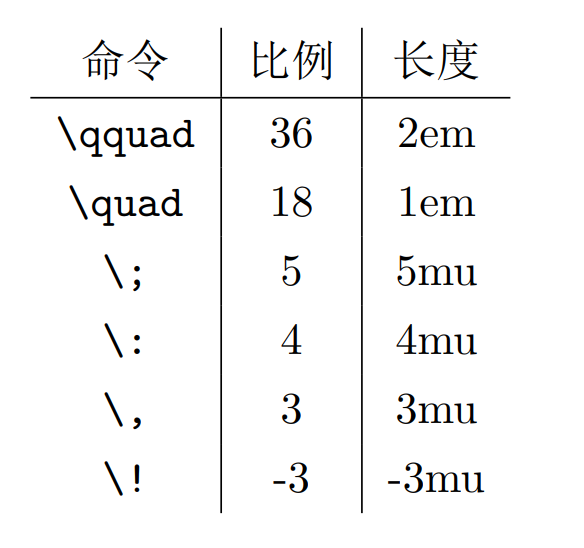
\includegraphics[width=0.5\textwidth]{pictures/spacing.png}}
    \parbox{0.5\textwidth}{
        内容内容内容内容内容内容内容内容内容内容内容内容内容内容内容内容内容内容内容内容内容内容内容内容内容内容内容内容内容内容内容内容内容内容内容内容内容内容内容内容内容内容内容内容内容内容内容内容内容内容内容内容内容内容内容内容内容内容内容内容内容内容内容内容内容内容内容内容内容
    }
}
之后的内容

之后的东西

\end{document}